
\begin{figure}
\centering
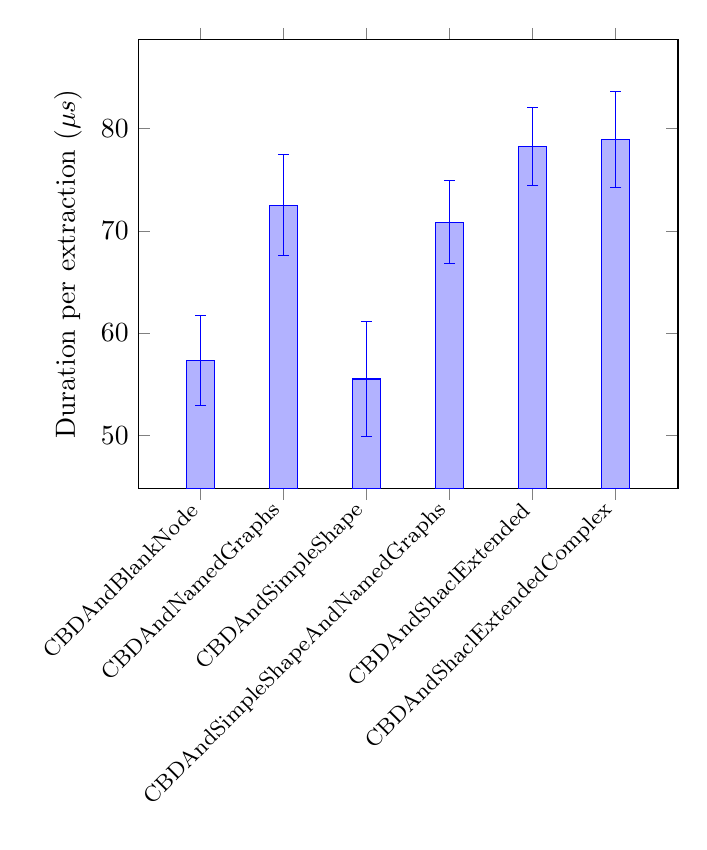
\begin{tikzpicture}
        \begin{axis}[
            ybar,
            enlargelimits=0.15,
            legend style={at={(0.5,-0.15)},
            anchor=north,legend columns=-1},
            ylabel={Duration per extraction ($\mu s$)},
            symbolic x coords={CBDAndBlankNode,CBDAndNamedGraphs,CBDAndSimpleShape,CBDAndSimpleShapeAndNamedGraphs,CBDAndShaclExtended,CBDAndShaclExtendedComplex},
            xtick=data,
            x tick label style={font=\footnotesize,rotate=45, anchor=east},
            nodes near coords align={horizontal},
        ]
            \addplot+[
                error bars/.cd,
                y dir=both,
                y explicit
            ] coordinates {
         (CBDAndBlankNode, 57.28933241657702) +- (0, 4.399687982971235)
         (CBDAndNamedGraphs, 72.52148850606409) +- (0, 4.97290233970496)
         (CBDAndSimpleShape, 55.501805795783895) +- (0, 5.615015619723464)
         (CBDAndSimpleShapeAndNamedGraphs, 70.83589491118653) +- (0, 4.068038426975957)
         (CBDAndShaclExtended, 78.22345534431719) +- (0, 3.8201542702061504)
         (CBDAndShaclExtendedComplex, 78.92954119439713) +- (0, 4.711264701511219)

             };
        \end{axis}
    \end{tikzpicture}
    \caption{Graph depicting performance of inband extraction algorithm}
\end{figure}
